\chapter{Implementation}
The suggested network forensic system is designed and implemented to detect and study the behavior of port scanning attack.
It is mainly divided in to three modules such as capture module, analysis module and virtualization module as mentioned in previous chapter.\\\\
The packet capturing system is used for capturing the packets and is installed in the network telescope.
It captures all kinds of the packets that pass through a given network interface and is implemented using C with libpcap library.
\begin{figure}[ht]
    \centering
	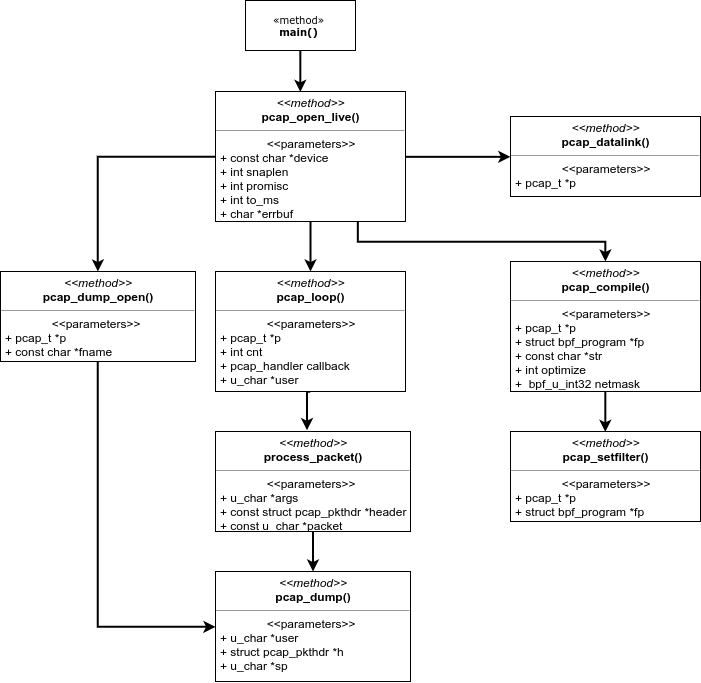
\includegraphics[width=10cm, height=12cm]{images/uml_packetcapture.png}
	\caption{Call Diagram of Packet Capturing System}
\end{figure}
\\\\
Figure 5.1 shows the important functions and how it is related to each other in packet capturing system.
We select the network device and open it using pcap\_openlive(), a function provided by libpcap library.
To capture all of the network traffic, we set up the network interface in to  promiscuous mode using promisc flag in pcap\_openlive.
This function returns an interface handler that will be used later when calling rest of the functions provided by libpcap.
Setting a filter involves three steps: constructing the filter expression, compiling the expression into a BSD Packet Filter (BSD) program and applying the filter.
We constructed the filter expression to remove the packets coming to server IP address from the captured dataset.
The expression is compiled using pcap\_compile() and inserted it into kernel calling the function pcap\_setfilter().
The pcap\_loop() is used to collect packets and process them.
This function calls a user defined function process\_packet() every time when there is a packet ready to read.
These packets are written to a capture file using the function pcap\_dump(). 
The captured files are stored in to hard disk and log files are rotated weekly using logrotate option in the UNIX.\\\\
The traffic collected by a network telescope provides a large dataset that needs to be analysed.
This can be achieved by a port scanning detection mechanism in the analysis module.
It is implemented separately in an another machine  which also runs ubuntu-16.04.4 using Python.
The Algorithm 1 gives a brief understanding about how port scanning detection mechanism was implemented.\\\\
We extract TCP and UDP port scans from the packets captured by the network telescope.
If a TCP packet is received, the port scanning detection algorithm examines for the multiple port scanning conditions.
The algorithm, for instance, initially inspects the half connect scanning (TCP SYN scanning) activity.
If the packet satisfies one of the port scanning criteria, it does not look for the remaining conditions.\\\\
The detection of several kinds of port scans  was implemented based on how each port scan really works and how host response to a packet. 
Section 2.2.3 explains common port scanning methods and how does it respond to the replies from target system.
Considering the working of different port scanning techniques, it utilize certain characteristics of particular protocols or platforms in order to better differentiate between open and closed ports.
We implemented functions to check the incoming packets fulfill the  condition of port scanning methods such as TCP connect scan, TCP half connect scan, UDP scan, Xmas scan, Null scan and FIN scan.
The detection of above mentioned port scanning mechanisms were implemented by using a buffer which stores each packet in that specific connection process until the next associated packet arrives. 
By examining the last packet in the buffer, we can decide up on the detection of port scans.
Moreover, for the purpose of analysis, we classified the port scans in to vertical and horizontal scans based on the analysis module design mentioned in Section 4.2.
Horizontal scans detection were implemented using Python dictionary, a  KeyValuePair$<$TKey, TValue$>$ Structure to store the source IP address as key and corresponding targeted IP addresses as values for each port scan.
Similarly we implemented the detection of vertical scans using a Python dictionary to store the source IP as key and corresponding targeted ports on a particular target system as values. 
Finally we stored these two buffers in JavaScript Object Notation (JSON), a lightweight data-interchange format for further analysis and plotting the graph.\\\\
\begin{algorithm}[H]
\For{each IPv$4$ packet in the captured file }{
    \uIf{the packet matches TCP }{
        \uIf{the packet fulfills three way handshake condition}{
           \uIf{the packet is TCP connect scan}{
                increment the occurrence of connect scan\;
                continue\;
            }
         }
         \uElseIf{the packet is TCP half connect scan}{
            increment the occurrence of half connect scan\;
            continue\;
         }
          \uElseIf{the packet does not fulfill three way handshake condition}{
         \uIf{the packet is FIN scan }{
             increment the occurrence of FIN scan\;
             continue\;
         }
         }
         \uElseIf{the packet is Xmas scan}{
             increment the occurrence of Xmas scan\;
             continue\;
         }
         \uElseIf{the packet is null scan }{
             increment the occurrence of null scan\;
             continue\;
         }
   }
   \uElseIf{the packet matches UDP}{
    increment the occurrence of UDP scan\;
    continue\;
    }
}
\caption{port scanning detection}
\end{algorithm}
\noindent
\\\\
However, Internet scanners use variety of methods to obscure the port scanning activity, thus evade the detection of port scanning mechanisms.
These obscuring methods are explained in Section 2.2.2.
One method to avoid the detection mechanism is to increase the time between successive port scanning packets.
To counter this method and to separate port scanning packets from other traffic, we looked for the port scans from the same source for 300 seconds.
Another method to avoid the detection is to use spoofed IP or IP decoys to hide the attacker's IP address.
We used two methods to combine the source IPs of port scans which seem coordinated as explained in Section 4.2.
We implemented the first method by combining the source IPs  with same first 3 bytes of the IP address. 
We implemented the second method by using IPWhois, a Python package focused on retrieving and parsing whois data for IPv4 addresses.
IPWhois package can be used to identify the autonomous system number (ASN) of each ISP, which was applied to combine the IPs based on the same ISP.
These two methods will give only an approximate solution which we use for comparison.\\\\
After the analysis part is finished, visualization module can be used to infer the relevant information from analysis module for further research.
The visualization module consist of graphs such as horizontal scan, vertical scan,  relationship between traffic rate and the time of the day and map which shows  geographical distribution of location of port scanning attacks as explained in Section 4.3.
It was implemented using several Python scripts.
We used Matplotlib: a plotting library for the Python to plot most of the graphs in this module.
The Python script to plot horizontal scan graph uses JSON file corresponding to horizontal scans from the previous stage as input.
JSON file consists of key value pairs with source system as key and targeted IP addresses as values.
While parsing through the JSON file, it is very straightforward to find the number of scans with number of destination IPs.
Vertical scan graph was also implemented using similar approach. 
We used several Python libraries to plot the graph showing relationship between  traffic rate of top 5 countries and local time of source of port scan.
GEOLITE: Geolocation library from MaxMind was used to identify the country of each IP address and Pytz: a library allows timezone calculations was used to convert the time of port scan from local timezone to timezone of source IP.
Moreover a heat map was generated to show the geographical distribution of location of port scanning attacks.
We used two main functions to produce this map.
First function uses the MaxMind library and databases to geolocate IP addresses and returns latitude and longitude location of IP address.
Second function takes the output from the first method as input and uses matplotlib basemap toolkit: a library for plotting 2D data on maps to generate the map.  
All the above mentioned scripts used the obtained results from the analysis module to display the corresponding information.
